\documentclass[11pt]{article}
\usepackage[margin=.8in]{geometry}
\usepackage{amsmath,amssymb,graphicx,hyperref}
\setlength{\parindent}{0pt}\setlength{\parskip}{6pt}
\begin{document}
\begin{center}{\Large What the constructed residual tells us about scalar labels}\\27 November 2026 --- unsigned local Lean component evidence\end{center}
\textbf{Actual conditional relation.}
Let \(h\ne0\) be an actual coordinate function and
\(\langle h\rangle=(\prod_i I_{P_i}^{n_i})J\).
Supply an \emph{exact} representation \(J=\prod_j I_{R_j}\) by actual
nonsingular rational points. Lean derives
\[
 \sum_i n_iP_i+\sum_jR_j=0,\qquad
 \sum_j R_j=-\sum_i n_iP_i.
\]
Thus the residual group sum is independent of the chosen function \(h\)
for fixed prescribed input points and levels. For a single residual point,
that point is determined. Multiple-point factorizations need not be fixed
(PCC-20261127-9326d2) [pcc:unverified].
\begin{center}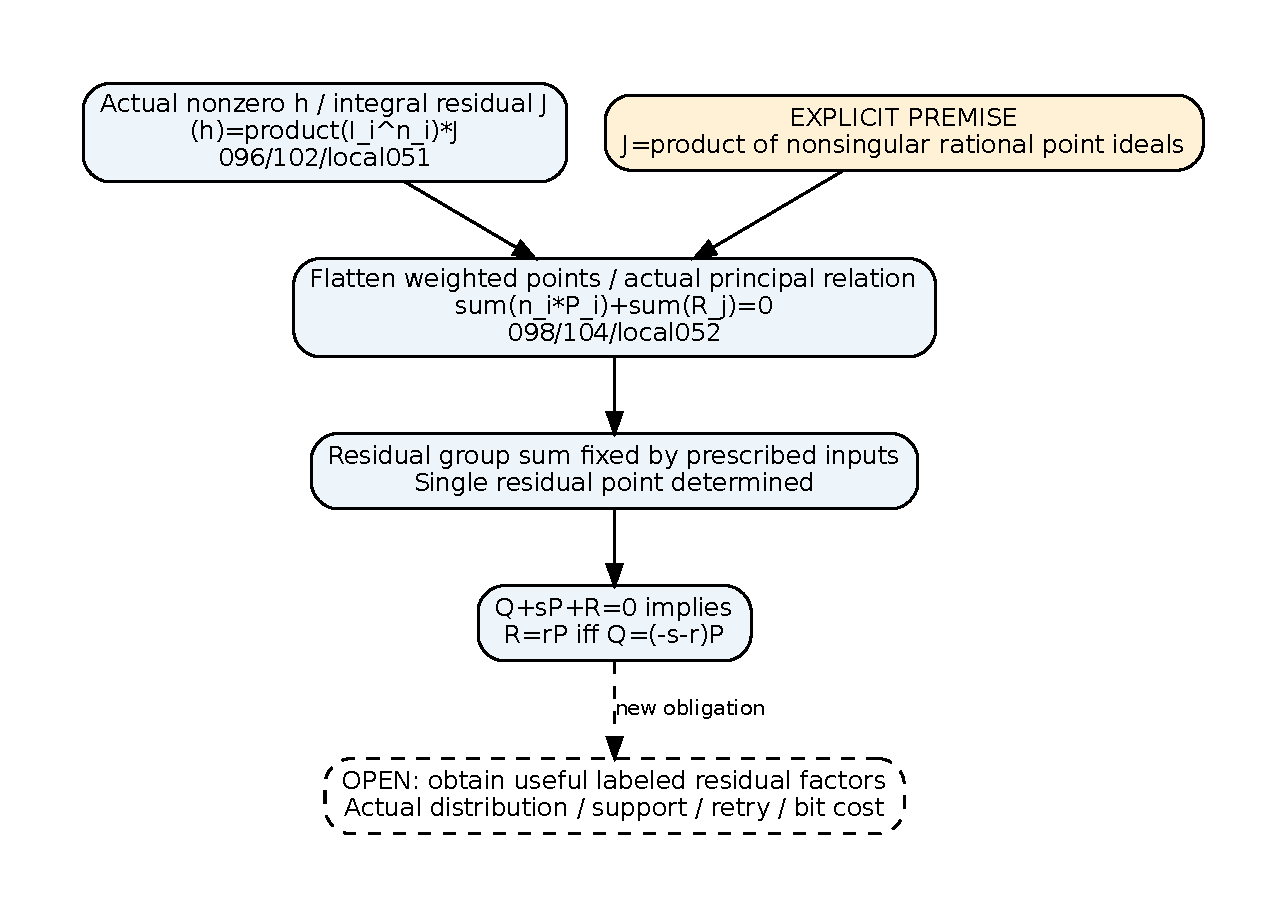
\includegraphics[height=4.6in,width=.98\linewidth,keepaspectratio]{residual-relation-dependencies-001.pdf}\end{center}
\textbf{Exact label equivalence.}
For integer labels and actual elliptic points, under \(Q+sP+R=0\),
\[
 R=rP\quad\Longleftrightarrow\quad Q=(-s-r)P.
\]
This equivalence does not compute either unknown logarithm [pcc:unverified].
\newpage
\begin{center}{\Large Proof map and implications for the next search}\end{center}
\textbf{Proof.}
Expand each actual point ideal power into a product indexed by
\(\operatorname{Fin}(n_i)\). Append the actual residual point family by a
disjoint index sum. The actual principal-ideal-to-point-sum theorem gives
the displayed elliptic relation, including repeated points, zero levels
and empty index families. Rearrangement determines the residual sum.
Applying the identity to two nonzero functions with the same prescribed
inputs gives sum invariance. For one residual point it gives that point
itself. Integer scalar addition and negation prove the label equivalence
[pcc:unverified].

\textbf{Lean map.}
All six declarations are in \texttt{OrientationActualGrowingRelation}:
\begin{center}\begin{tabular}{ll}
Declaration&Checked scope\\
\texttt{weighted\_point\_sum}&actual principal product of weighted point ideals\\
\texttt{weighted\_residual\_sum}&actual factorization plus explicit residual product\\
\texttt{residual\_sum\_determined}&negative prescribed weighted input sum\\
\texttt{residual\_sum\_independent}&two actual functions, same prescribed inputs\\
\texttt{single\_residual\_determined}&one actual residual point ideal\\
\texttt{residual\_scalar\_iff}&\(Q+sP+R=0\), integer labels
\end{tabular}\end{center}
Source098/build104/local052 checks258 printed statements, six new since252,
exit zero, zero warnings and standard printed foundations;354 exact input
bindings checked. Failed097/build103 had two dependent-sum normalization
errors, so its whole candidate was rejected. Repaired098 explicitly rewrites
the sums to constant point summands; mathematical premises are unchanged.
Raw failed source, output and exit remain preserved [pcc:unverified].

\textbf{Scope.}
The rational nonsingular residual point-product representation is an explicit
premise. It is not inferred from the integral residual's degree bound.
No unknown scalar label is declared known. The invariance concerns the group
sum, not every possible multi-point factorization. It does not establish a
generic runtime lower bound, exclude adaptive input support, or exclude a
higher-degree smoothness strategy. All evidence is unsigned local, outside
historical shared Transport53/57 audit/fresh.

\textbf{Next discriminating obligation.}
Establish the weighted scalar congruence with explicit target multiplicity
and unit condition modulo subgroup order. Then construct a public procedure
that obtains independently useful labeled residual factors. Its actual
class-conditioned success probability, support selection, retries and full
bit cost must be derived. A random-divisor smoothness heuristic alone does
not establish the distribution of the actual coefficient-kernel sampler.

\textbf{Sources checked.}
Actual NormGroupBridge principal-product point sum and target scalar proof;
existing fixed-point residual-class invariant; public Mathlib dependent and
disjoint finite sums/products; elementary elliptic group identities. These
are standard algebraic methods, without novelty claims. KB unavailable in
this runtime; exact source fallback used. Protocol017 and continuation027
preserve the next action.
\end{document}
